\section{Mappe Ricorsive}%
\label{sub:Mappe Ricorsive}
Ricordiamo che una mappa ricorsiva è definita da:
\[
    \vect{x}_{n+1} = G(\vect{x}_n) \qquad \vect{x}_n \in \mathbb{R}^n; \qquad G:\mathbb{R}^n\to \mathbb{R}^n
.\] 
\begin{enumerate}
    \item La mappa è invertibile se $\exists \ G^{-1}$.
    \item La mappa è $C^r$ se esistono e sono continue le derivate\sidenote{\scriptsize Intese come parziali in più dimensioni} di $G$ fino all'ordine $r$.
\end{enumerate}
Se valgono la $1)$ e la $2)$ allora si ha un \textbf{Diffeomorfismo} $C^r$.
\subsection{Orbita per mappa ricorsiva invertibile}%
\label{sub:Orbita per mappa ricorsiva invertibile}
Se la mappa è invertibile allora preso un punto $\vect{x}_0$ è possibile muoversi verso destra (con $G$) o verso sinistra con $G^{-1}$.
\[
    \ldots, \ G^{-1}(\vect{x}_0), \ G^{-1}(\vect{x}_0), \ \vect{x}_0, \ G(\vect{x}_0), \ G^2(\vect{x}_0), \ \ldots
.\] 
\begin{exmp}[Mappa lineare]
    \[
        x_{n+1} = a x_n \qquad a \in \mathbb{R} - \left\{0\right\}
    .\] 
    Questa mappa è invertibile: basta spostare il parametro $a$ a sinistra per ricavare la preimmagine.
\end{exmp}
\noindent
Le mappe più studiate sono quelle non invertibili, questo perché al variare dei loro parametri si possono generare dei comportamenti particolari (caos).\\
Ci sono casi in cui anche le mappe all'apparenza invertibili possono generare situazioni complicate, ad esempio quelle che presentano un modulo come vedremo negli esempi di questa sezione.
\subsection{Orbita per mappa ricorsiva non invertibile}%
\label{sub:Orbita per mappa ricorsiva non invertibile}
Preso un punto $\vect{x}_0$ per una mappa non invertibile è possibile spostarsi soltanto verso destra tramite la $G$.
\[
    \vect{x}_0, \ G(\vect{x}_0), \ G^2(\vect{x}_0), \ \ldots
.\] 
\begin{exmp}[Mappa logistica]
    \[
        x_{n+1} = 3.5 x_n \left(1- x_n\right) \qquad x_n \in \left[0,1\right]
    .\] 
    Questa mappa non è invertibile: la preimmagine non è univoca (un'equazione del secondo grado ha due soluzioni).
\end{exmp}
\noindent
\begin{exmp}[Mappa di Bernoulli]
    \[
	x_{n+1}=2x_n \quad \text{mod}(1)
    .\] 
    Questa mappa è parente della shift-map poiché, scegliendo di rappresentare $x$ in base due, la mappa agisce allo stesso modo sui coefficienti della espansione (di base due) di come agiva con i simboli la shift map.
    \marginpar{
        \captionsetup{type=figure}
            \incfig{4_1}
        \caption{\scriptsize Mappa di Bernoulli, si vede come la linea rossa non rappresenti una funzione iniettiva: non può essere invertibile.}
        \label{fig:4_1}
    }\\
    L'operazione di modulo $1$ invece si occupa di traslare in $[0,1]$ il punto $x_{n+1}$ ogni volta che esce dall'intervallo a causa all'applicazione della mappa. \\
    L'operazione di traslazione avviene tramite un intero $n$ tale che:
    \[
	n = \text{min}(k \in \mathbb{Z}): \ 0 \le x+n \le 1
    .\] 
    Pur essendo lineare (all'apparenza) questa mappa può esibire un comportamento complesso. La presenza del modulo infatti fa si che la mappa non sia invertibile, come si può vedere in figura \ref{fig:4_1}.
\end{exmp}
\noindent
    \begin{exmp}[Circle Rotation Map]
	Prendiamo una classe di mappe generale del seguente tipo:
        \[
	    x_{n+1} = G(x_n) \qquad x_n \in S_1
        .\] 
	$S_1$ rappresenta il cerchio di raggio unitario, quindi i punti della mappa appartengono tutti al cerchio e sono rappresentati da una variabile: l'angolo di rotazione $x\cdot 2\pi$ (con $x \in \left[0,1\right]$).
	\marginpar{
	    \captionsetup{type=figure}
	        \incfig{4_2}
	    \caption{\scriptsize Rappresentazione della Circle Rotation Map.}
	    \label{fig:4_2}
	}\\
	La Circle Rotation Map è un caso particolare di queste mappe, ovvero:
	\[
	    x_{n+1}=x_n+\alpha  \quad \text{mod}(1); \qquad \alpha\in [0,1[
	.\] 
	La caratteristica principale di questa mappa è che può essere:
	\begin{itemize}
	    \item \textbf{$k$-periodica} se $\alpha$ razionale: le orbite degli $x_n$ si richiudono.
	    \item \textbf{Quasi periodica} se $\alpha$ irrazionale: i punti della mappa si distribuiscono uniformemente sul cerchio unitario (questo è il caso mostrato in figura \ref{fig:4_2}).
	\end{itemize}
	La mappa è sempre invertibile. 
\end{exmp}
\noindent
\begin{exmp}[Mappa di Arnold]
        \[
	    x_{n+1} = x_n + \omega  - \frac{k}{2\pi}\sin (2\pi x_n) \qquad \text{mod}(1) 
        .\] 
	$k, \omega$ sono costanti e $k>0$, la mappa non è lineare a causa della presenza del $\sin$.\\
	Il parametro $\omega$ può essere interpretato come il rapporto tra due frequenze: una intrinseca del sistema ed una forzante esterna.
	\[
	    \omega  \sim \frac{\omega_{\text{int}}}{\omega_{\text{ext}}}; \qquad \omega \in \left[0,1\right]
	.\]
	La mappa mostra le seguenti peculiarità:
	\begin{itemize}
	    \item $0\le k\le 1$: la mappa di comporta come la Circle Map, presenta orbite periodiche o quasi periodiche a seconda della razionalità di $\omega$. 
	    \item $k>1$: la mappa può esibire comportamenti caotici.
	\end{itemize}
	Nel caso di $k=1$ la mappa inizia a riscontrare alcune "anomalie", è il valore per il quale iniziano a rompersi le "lingue di Arnold".
\end{exmp}
\noindent
\begin{ex}[Sulla mappa di Arnold]
       Dimostrare che la mappa di Arnold è invertibile se $0\le k\le 1$.\\
       \textbf{Soluzione}:
       \marginpar{
           \captionsetup{type=figure}
           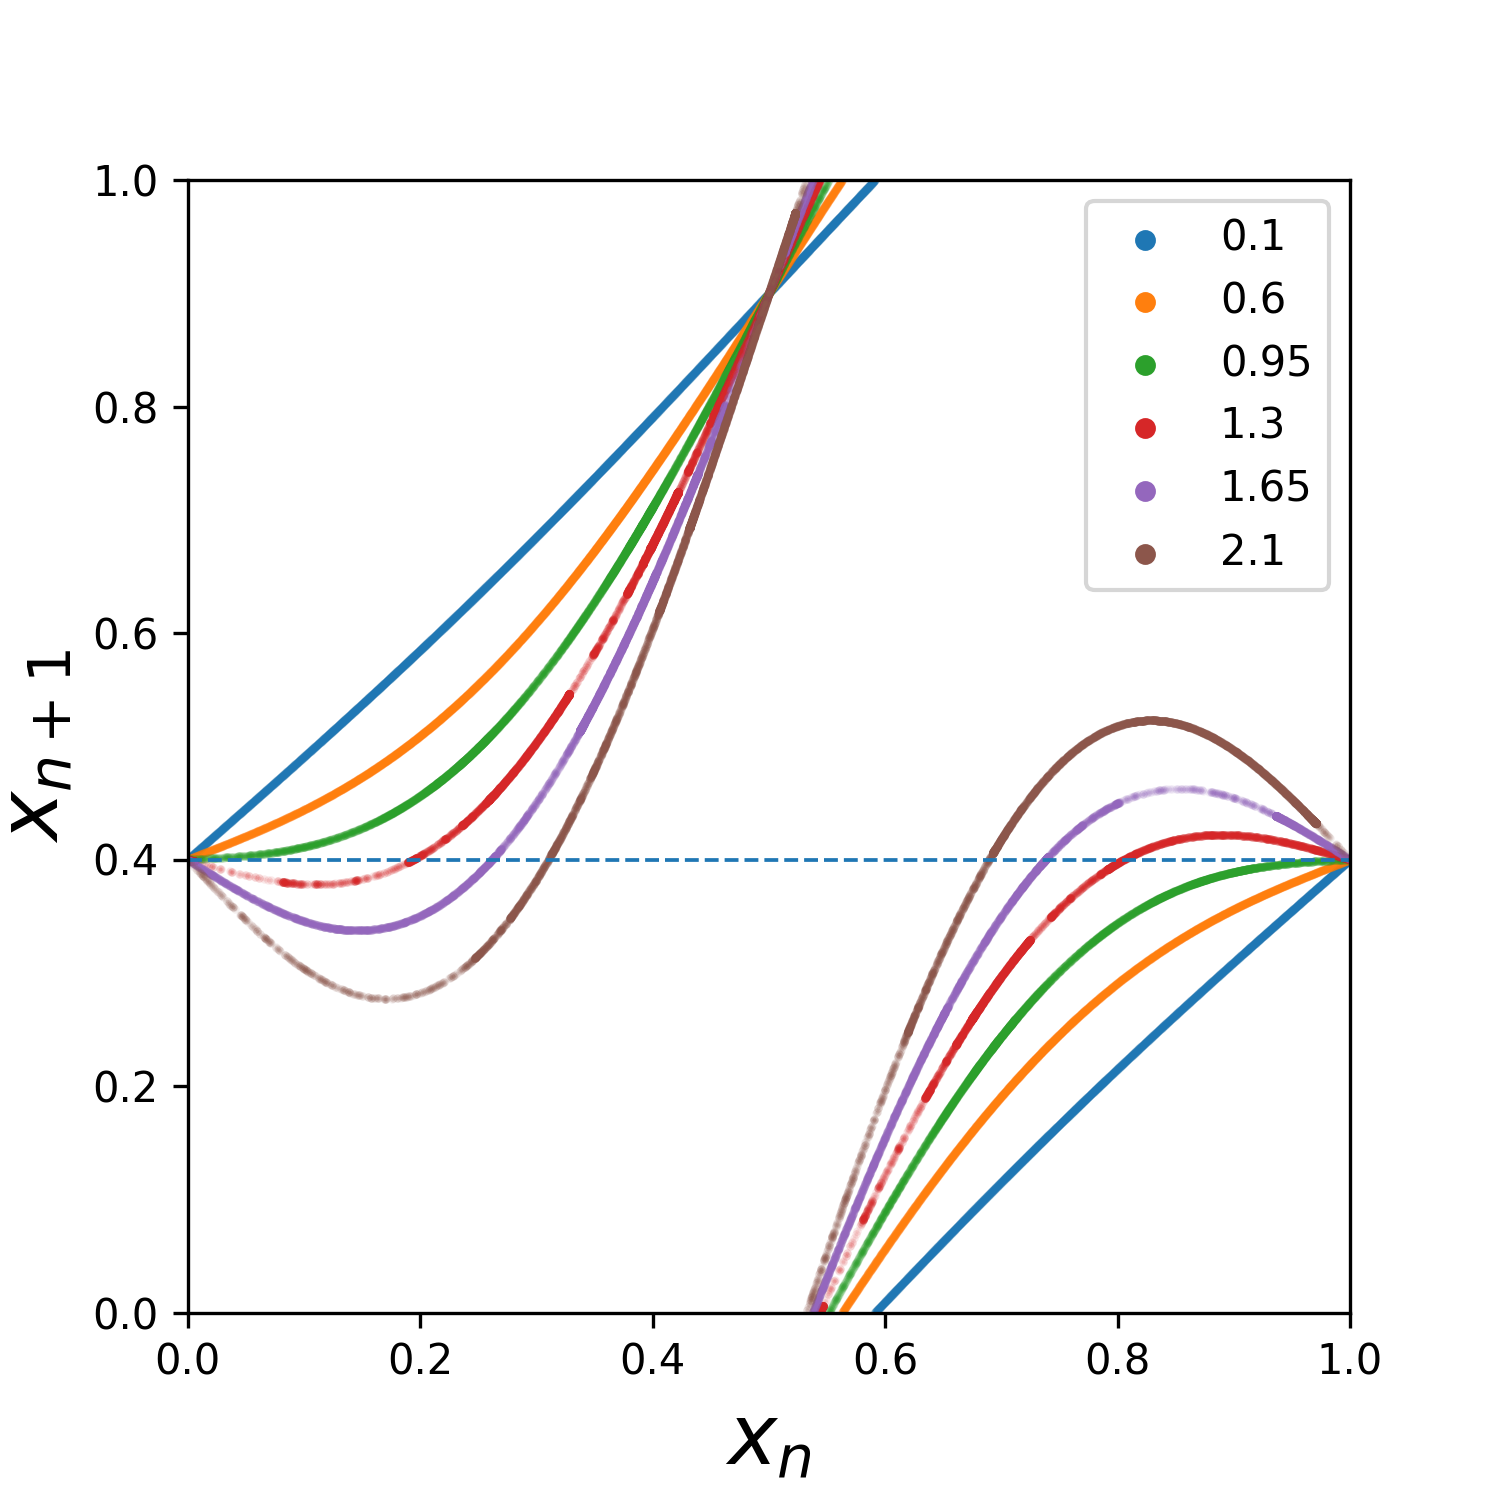
\includegraphics[width=\marginparwidth]{figures/4_3_py.png}
	   \caption{\scriptsize Mappa di Arnold al variare di $k$ con $\omega  = 0.4$ fissato.}
           \label{fig:4_3_py-png}
       }
       Come possiamo vedere in figura \ref{fig:4_3_py-png} la mappa non è invertibile per tutti i valori di $k$. \\
       Prendiamo ad esempio la mappa con $k=0.1$ e valutiamo\sidenote{\scriptsize Questa corrisponde (circa) alla circle rotation map} il punto $x_n=0$: la linea blu in figura \ref{fig:4_3_py-png}, che rappresenta la mappa, a destra di questo punto vale $\omega+\epsilon$, a sinistra di questo punto vale $\omega-\epsilon$. La pendenza della curva in questo punto è quindi positiva.\\
       La presenza della perturbazione oscillante fa si che i due "rami" della mappa si avvicinino l'un l'altro "distorcendosi", di conseguenza se la perturbazione è abbastanza forte è possibile che in un punto tra $0$ e $1$ il ramo in alto e quello in basso abbiano la stessa $x_{n+1}$: si perde l'iniettività e quindi l'invertibilità.\\
       Nel grafico la perdita di iniettività si ha quando la mappa oltrepassa la linea tratteggiata (che rappresenta la separatrice tra i rami).\\
       Per capire quando questo succede possiamo studiare la pendenza della mappa nei pressi di $x_n = 0$ (considerandola di fatto come una funzione continua).
       \[
	   x_{n+1} = x_n + \omega + k x_n = (1-k) x_n + \omega
       .\] 
       Se in un intorno (destro) di questo punto la pendenza della curva è negativa allora significa che la mappa è scesa sotto $\omega$ e quindi ha perso l'iniettività: deve essere $k\le 1$ per avere pendenza positiva.
\end{ex}
\noindent

